%%%%%%%%%%%%%%%%%%%%%%%%%%%%%%%%%%%%%%%%%%%%%%%%%%%%%%%%%%%%%%%%
%%                                                            %%
%%   essentialsOfLatin, Italian translation 2017              %%
%%                                                            %%
%% From:  Henry C. Pearson, Essentials Of Latin For Beginners %%
%%        (1915, New York, American Book Company)             %%
%%                                                            %%
%%    https://archive.org/details/essentialslatin04peargoog   %%
%%                                                            %%
%% Translated by g.p.ciceri <gp.ciceri@gmail.com>             %%
%% ---------------------------------------------------------- %%
%% This translation is Licensed under                         %%
%% Creative Commons Attribution-ShareAlike 4.0 International  %%
%% https://creativecommons.org/licenses/by-sa/4.0/            %%
%%                                                            %%
%%%%%%%%%%%%%%%%%%%%%%%%%%%%%%%%%%%%%%%%%%%%%%%%%%%%%%%%%%%%%%%%

% āēīōū
% ăĕĭŏŭ




\documentclass[nols]{tufte-handout}

%\geometry{showframe} % display margins for debugging page layout

\usepackage{fontspec}
\usepackage{ifxetex}
\setmainfont[Path=./fonts/palatino-linotype/, ItalicFont=palai.ttf, BoldFont=palab.ttf]{pala.ttf}


% \defaultfontfeatures{Mapping=tex-text}
% \setromanfont[Path=./fonts/TeX-Gyre-Schola/,Mapping=tex-text]{TeX Gyre Schola}
% \setsansfont[Path=./fonts/TeX-Gyre-Heros/,Scale=MatchLowercase,Mapping=tex-text]{TeX Gyre Heros}
% \setmonofont[Path=./fonts/TeX-Gyre-Cursor/,Scale=MatchLowercase]{TeX Gyre Cursor}

\usepackage{lipsum}
\usepackage{url}
\usepackage{longtable}
\usepackage{stackengine}

\usepackage{graphicx} % allow embedded images
  \setkeys{Gin}{width=\linewidth,totalheight=\textheight,keepaspectratio}
  \graphicspath{{graphics/}} % set of paths to search for images
\usepackage{amsmath}  % extended mathematics
\usepackage{booktabs} % book-quality tables
\usepackage{units}    % non-stacked fractions and better unit spacing
\usepackage{multicol} % multiple column layout facilities
\usepackage{lipsum}   % filler text
\usepackage{fancyvrb} % extended verbatim environments
  \fvset{fontsize=\normalsize}% default font size for fancy-verbatim environments

% Standardize command font styles and environments
\newcommand{\doccmd}[1]{\texttt{\textbackslash#1}}% command name -- adds backslash automatically
\newcommand{\docopt}[1]{\ensuremath{\langle}\textrm{\textit{#1}}\ensuremath{\rangle}}% optional command argument
\newcommand{\docarg}[1]{\textrm{\textit{#1}}}% (required) command argument
\newcommand{\docenv}[1]{\textsf{#1}}% environment name
\newcommand{\docpkg}[1]{\texttt{#1}}% package name
\newcommand{\doccls}[1]{\texttt{#1}}% document class name
\newcommand{\docclsopt}[1]{\texttt{#1}}% document class option name
\newenvironment{docspec}{\begin{quote}\noindent}{\end{quote}}% command specification environment

% concetti morfosintattici
\usepackage{xspace} 
\newcommand{\noun}{\textsc{sostantivo}\xspace}
\newcommand{\nouns}{\textsc{sostantivi}\xspace}
\newcommand{\adject}{\textsc{aggettivo}\xspace}
\newcommand{\adjects}{\textsc{aggettivi}\xspace}
\newcommand{\gnumber}{\textsc{numero}\xspace}
\newcommand{\gnumbers}{\textsc{numeri}\xspace}
\newcommand{\gender}{\textsc{genere}\xspace}
\newcommand{\genders}{\textsc{generi}\xspace}
\newcommand{\gcase}{\textsc{caso}\xspace}
\newcommand{\gcases}{\textsc{casi}\xspace}
\newcommand{\tense}{\textsc{tempo}\xspace}
\newcommand{\mood}{\textsc{modo}\xspace}
\newcommand{\gverb}{\textsc{verbo}\xspace}
\newcommand{\gverbs}{\textsc{verbi}\xspace}
\newcommand{\adjective}{\textsc{aggettivo}\xspace}
\newcommand{\nom}{\textsc{nom}\xspace}
\newcommand{\gen}{\textsc{gen}\xspace}
\newcommand{\dat}{\textsc{dat}\xspace}
\newcommand{\acc}{\textsc{acc}\xspace}
\newcommand{\voc}{\textsc{voc}\xspace}
\newcommand{\abl}{\textsc{abl}\xspace}
\newcommand{\gexit}{\textsc{uscita}\xspace}
\newcommand{\gexits}{\textsc{uscite}\xspace}
\newcommand{\declinazione}{\textsc{declinazione}\xspace}
\newcommand{\masc}{\textsc{maschile}\xspace}
\newcommand{\femm}{\textsc{femminile}\xspace}
\newcommand{\neut}{\textsc{neutro}\xspace}

\newcommand{\indic}{\textsc{indicativo}\xspace}
\newcommand{\imper}{\textsc{imperativo}\xspace}
\newcommand{\gcong}{\textsc{congiuntivo}\xspace}
\newcommand{\ott}{\textsc{ottativo}\xspace}
\newcommand{\partic}{\textsc{participio}\xspace}
\newcommand{\infin}{\textsc{infinito}\xspace}

\newcommand{\pres}{\textsc{presente}\xspace}
\newcommand{\imperf}{\textsc{imperfetto}\xspace}
\newcommand{\aor}{\textsc{aoristo}\xspace}
\newcommand{\fut}{\textsc{futuro}\xspace}
\newcommand{\perf}{\textsc{perfetto}\xspace}
\newcommand{\pperf}{\textsc{piuccheperfetto}\xspace}

\newcommand{\sing}{\textsc{singolare}\xspace}
\newcommand{\plur}{\textsc{plurale}\xspace}
\newcommand{\dual}{\textsc{duale}\xspace}

\newcommand{\si}{\textsc{sing}\xspace}
\newcommand{\pl}{\textsc{plur}\xspace}
\newcommand{\du}{\textsc{dual}\xspace}

\newcommand{\att}{\textsc{attivo}\xspace}
\newcommand{\med}{\textsc{medio}\xspace}
\newcommand{\pass}{\textsc{passivo}\xspace}
\newcommand{\medpass}{\textsc{medio-passivo}\xspace}


% italianitudini
\renewcommand{\figurename}{Figura}
\renewcommand{\tablename}{Tabella}
\renewcommand{\contentsname}{Indice}

% fix per un qualche problema
\ifxetex
  \newcommand{\textls}[2][5]{%
    \begingroup\addfontfeatures{LetterSpace=#1}#2\endgroup
  }
  \renewcommand{\allcapsspacing}[1]{\textls[15]{#1}}
  \renewcommand{\smallcapsspacing}[1]{\textls[10]{#1}}
  \renewcommand{\allcaps}[1]{\textls[15]{\MakeTextUppercase{#1}}}
  \renewcommand{\smallcaps}[1]{\smallcapsspacing{\scshape\MakeTextLowercase{#1}}}
  \renewcommand{\textsc}[1]{\smallcapsspacing{\textsmallcaps{#1}}}
\fi

% too many float...
\extrafloats{100}
% āēīōū
% ăĕĭŏŭ

\title{Essentials Of Latin. Elementi di Latino. \newline Lezione IV - Prima Coniugazione, Indicativo Presente di amō. Il caso Accusativo.}

\author[gpciceri]{a cura di Milagathòs: Milo's help to enjoy humanities.}

\date{24 Gennajo 2017} % without \date command, current date is supplied


\begin{document}

\hyphenation{co-niu-ga-zio-ne}

\maketitle% this prints the handout title, author, and date

\begin{marginfigure}[-2.5cm]
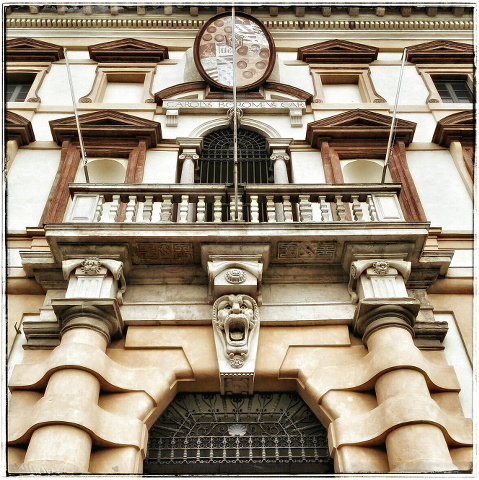
\includegraphics{smallthumb-lesson_I.jpeg}
\setfloatalignment{b}
\end{marginfigure}


\begin{abstract}
\noindent
Queste lezioni riprendono il testo introduttivo al Latino di Pearson\cite{pearson1915}, del quale seguono la numerazione; la struttura di ogni lezione è piuttosto regolare: inizia con \textsc{cenni di morfologia e di sintassi latina}, seguita da un \textsc{piccolo vocabolario} per il lessico; ci sono infine vari \textsc{esercizi} di traduzione e di composizione latina.

\bigskip
\noindent
Lezione IV - Prima Coniugazione, Indicativo Presente di amō, il caso Accusativo, concordanza tra soggetto e verbo, vocabolario, esercizi.
\end{abstract}

%\printclassoptions
% āēīōū
% ăĕĭŏŭ


\newthought{43. Indicativo Presente del verbo amare}
\begin{fullwidth}
\begin{table}[!htbp]
  \centering
  \begin{tabular}{l l l}
    %\toprule
	\multicolumn{3}{c}{\textbf{amō}, \textit{io amo}}\\
	& \multicolumn{1}{c}{\textsc{Singolare}} & \multicolumn{1}{c}{\textsc{Uscite}}\\
	
    \textsc{1.} & am\textbf{ō}, \textit{io amo} & \textbf{-ō} (o \textbf{-m}), \textit{io} \\
    \textsc{2.} & amā\textbf{s}, \textit{tu ami}   & \textbf{-s}, \textit{tu} \\
    \textsc{2.} & ama\textbf{t}, \textit{egli ama}  & \textbf{-t}, \textit{egli} \\
	
	\multicolumn{3}{c}{\textemdash}\\
	& \multicolumn{1}{c}{\textsc{Plurale}} & \multicolumn{1}{c}{\textsc{Uscite}}\\
	
	\textsc{1.} & amā\textbf{mus}, \textit{noi amiamo} & \textbf{-mus}, \textit{noi} \\
    \textsc{2.} & amā\textbf{tis}, \textit{voi amate}   & \textbf{-tis}, \textit{voi } \\
    \textsc{2.} & ama\textbf{nt}, \textit{essi amano}  & \textbf{-nt}, \textit{essi} \\
		
    %\bottomrule
  \end{tabular}
  %\caption[bottom]{Prima Declinazione. \textbf{stella, -ae}, f.}
  \label{tab:normaltab}
  %\zsavepos{pos:normaltab}
\end{table}
\end{fullwidth}
\sidenote{le uscite sono valide per tutti i tempi, tranne che per l'indicativo perfetto.}

\newthought{Osservazione}
\begin{itemize}
\item[\textsc{1.}] Le uscite si agganciano alla radice \textbf{amā-}, la cui vocale finale \textbf{ā} cade prima dell'uscita \textbf{ō} della prima persona singolare, ed è accorciata (ă) prima di \textbf{-t, -nt}.
\item[\textsc{2.}] La persona e il numero di un verbo latino sono indicate chiaramente dall'uscita, senza aver bisogno di usare un pronome.   
\end{itemize}

\newthought{44.} Impara a memoria il significato dei verbi seguenti e coniugali come \textbf{amō}:

\begin{multicols}{2}
    \noindent \hangindent=1em \textbf{pugnō}, \textit{io combatto}.  \\
    \noindent \hangindent=1em \textbf{vocō}, \textit{io chiamo}.  \\
	\noindent \hangindent=1em \textbf{culpō}, \textit{io accuso}.  \\
	\noindent \hangindent=1em \textbf{laudō}, \textit{io lodo, apprezzo}.  \\
	
	
\end{multicols}

\newpage

\newthought{45. Frasi Modello.} Esamina le seguenti frasi:
\begin{itemize}
\item[\textsc{1.}] \textbf{Regina nautam laudat}, \textit{la regina loda il marinaio}.  
\item[\textsc{2.}] \textbf{Reginae nautam laudant}, \textit{le regine lodano il marinaio}.    
\item[\textsc{3.}] \textbf{Nautam laudant}, \textit{essi lodano il marinaio}.    
\item[\textsc{3.}] \textbf{Nautam laudamus}, \textit{noi lodiamo il marinaio}.    
\end{itemize}
Da questi esempi osserviamo che \\
\begin{itemize}
\item[\textsc{1.}] L'oggetto diretto del verbo, cioè quello direttamente interessato dall'azione del verbo, viene espresso in caso accusativo. 
\item[\textsc{2.}] Quando il soggetto è un nome, il verbo è alla terza persona.  
\item[\textsc{3.}] Quando il soggetto non è un nome, non è obbligatorio venga espresso con una parola apposita.  
\item[\textsc{4.}] Il verbo è alla stessa \textit{persona} e \textit{numero} del soggetto.  
\end{itemize}

\newthought{46. Regole di Sintassi.} 
\begin{itemize}
\item[\textsc{1. Concordanza del Verbo con il Soggetto.}] Il verbo concorda con il suo soggetto in \textit{persona} e \textit{numero}. 
\item[\textsc{2. Complemento Oggetto (Oggetto Diretto).}] L'oggetto diretto di un verbo transitivo viene espresso in caso accusativo.  
\end{itemize}Il caso Genitivo. Il genitivo è usato per specificare (limitare) o definire il significato di un nome.

\newthought{47. Vocabolario}

\begin{multicols}{2}
    \noindent \hangindent=1em \textbf{agricola, -ae}, f., \textit{moneta}.  \\
    \noindent \hangindent=1em \textbf{nauta, -ae}, f., \textit{vita}.  \\
	
	\noindent \hangindent=1em \textbf{Italia, -ae}, f., \textit{Grecia}.  \\
	\noindent \hangindent=1em \textbf{Roma, -ae}, f., \textit{Europa}.  \\
	
	\noindent \hangindent=1em \textbf{inopia, -ae}, f., \textit{figlia}.  \\

	\noindent \hangindent=1em \textbf{fida, -ae}, agg.f. \textit{nuova}.  \\
	\noindent \hangindent=1em \textbf{superba, -ae}, agg.f. \textit{piccola}.  \\
	
	\noindent \hangindent=1em \textbf{amō}, \textit{io amo, mi piace}.  \\
	\noindent \hangindent=1em \textbf{pugnō}, \textit{io combatto}.  \\
    \noindent \hangindent=1em \textbf{vocō}, \textit{io chiamo}.  \\
	\noindent \hangindent=1em \textbf{culpō}, \textit{io accuso}.  \\
	\noindent \hangindent=1em \textbf{laudō}, \textit{io lodo, apprezzo}.  \\
	
	\noindent \hangindent=1em \textbf{cur}, avv.interr. \textit{perché?}.  \\
	
	\noindent \hangindent=1em \textbf{in}, prep con \abl, \textit{in, su}.  \\
	
\end{multicols}
% āēīōū
% ăĕĭŏŭ

\newthought{48. Esercizi di Ripasso}
\\
\textsc{I.} \quad
\textsc{1.}~Graeciae insulae sunt parvae. \quad
\textsc{2.}~Pecunia mea. \quad
\textsc{3.}~Suntne copiae patriae tuae magnae? \quad
\textsc{4.}~Feminae filiae non semper bonae sunt. \quad
\textsc{5.}~Est copia pecuniae. \quad
\textsc{6.}~Pulchrae sunt Europae viae. \quad
\textsc{7.}~Estne fabula nova?
\\
\textsc{II.} \quad
\textsc{1.}~Dove siete? \quad
\textsc{2.}~Non sono belle le figlie della regina? \quad
\textsc{3.}~Lei è piccola. \quad
\textsc{4.}~O regina, dov'è tua figlia? \quad
\textsc{5.}~Noi siamo; tu sei.


\newthought{49. Esercizi}
\\
\textsc{I.} \quad
\textsc{1.}~Pugnatis; pugnat; pugnamus. \quad
\textsc{2.}~Vocas; vocantne?; vocatisne? \quad
\textsc{3.}~Cur agricolas culpamus? \quad
\textsc{4.}~In Italia inopia est pecuniae. \quad
\textsc{5.}~Laudantne nautas? \quad
\textsc{6.}~Superbas feminas non amamus. \quad
\textsc{7.}~Reginae nautas non laudamus. \quad
\textsc{8.}~Superbae in Gallia sunt puellae. \quad
\textsc{9.}~Ubi sunt agricolarum filiae? \quad
\textsc{10.}~Cur nautam culpat? \quad
\textsc{11.}~Rosae magnae et pulchrae sunt in mea patria. \quad
\textsc{12.}~Agricolae inopiam pecuniae non amant.
\\
\textsc{II.} \quad
\textsc{1.}~Noi accusiamo; ella loda; voi chiamate. \quad
\textsc{2.}~Essi combattono; tu chiamo, noi combattiamo. \quad
\textsc{3.}~Ci sono belle rose in Italia. \quad
\textsc{4.}~Perché accusi il marinaio? \quad
\textsc{5.}~La ragazza chiama le figlie del marinaio. \quad
\textsc{6.}~L'Italia è un paese dell'Europa. \quad


\begin{figure}[!b]
  %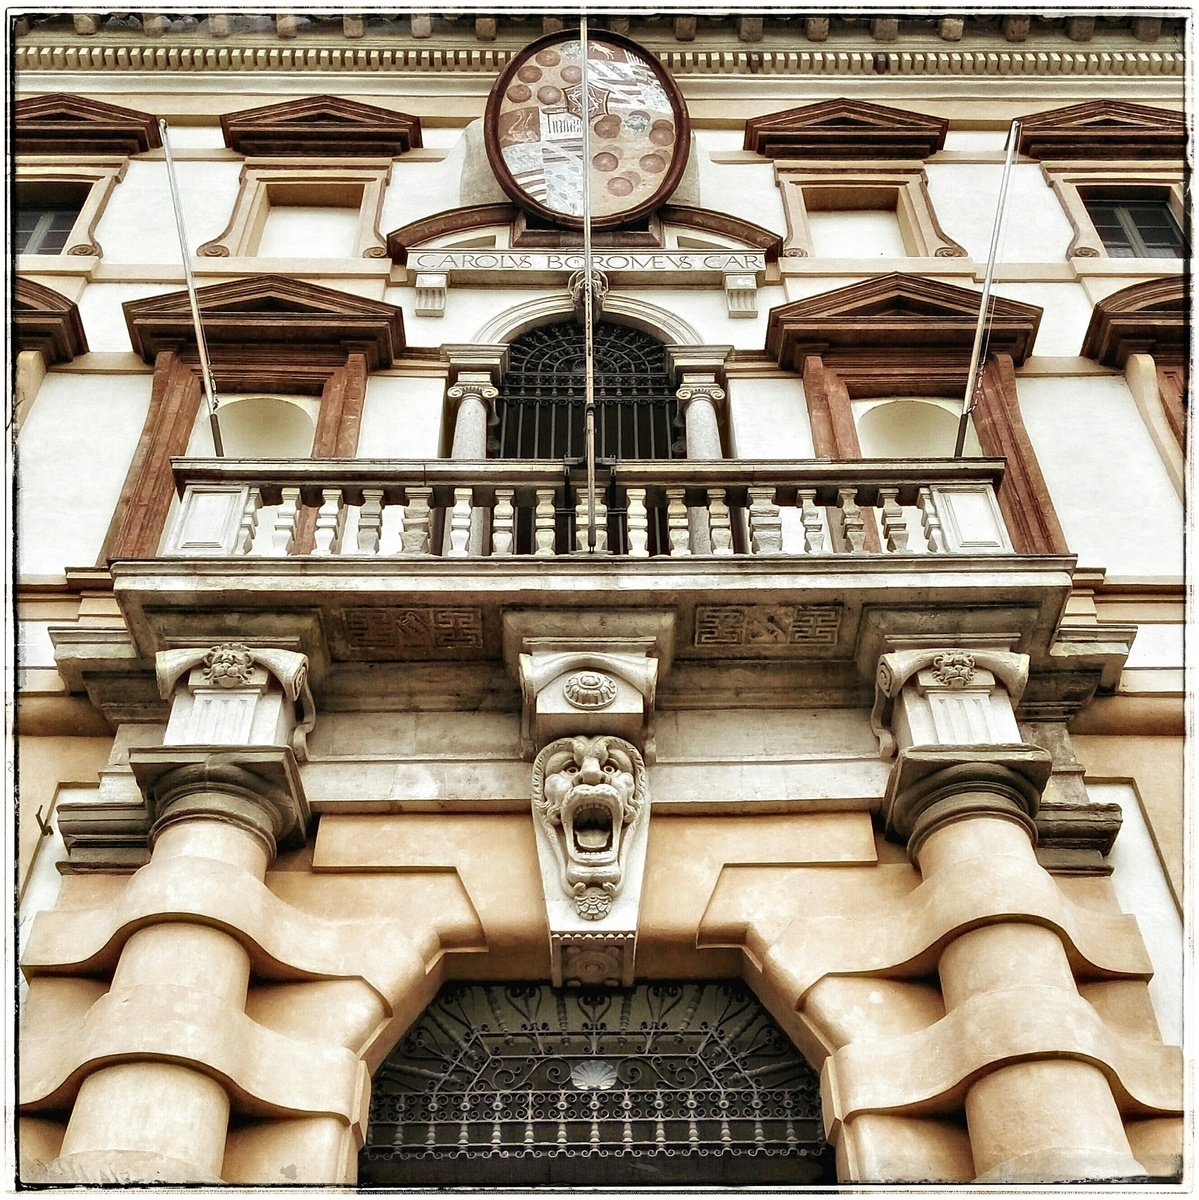
\includegraphics{thumb-lesson_I.jpeg}
  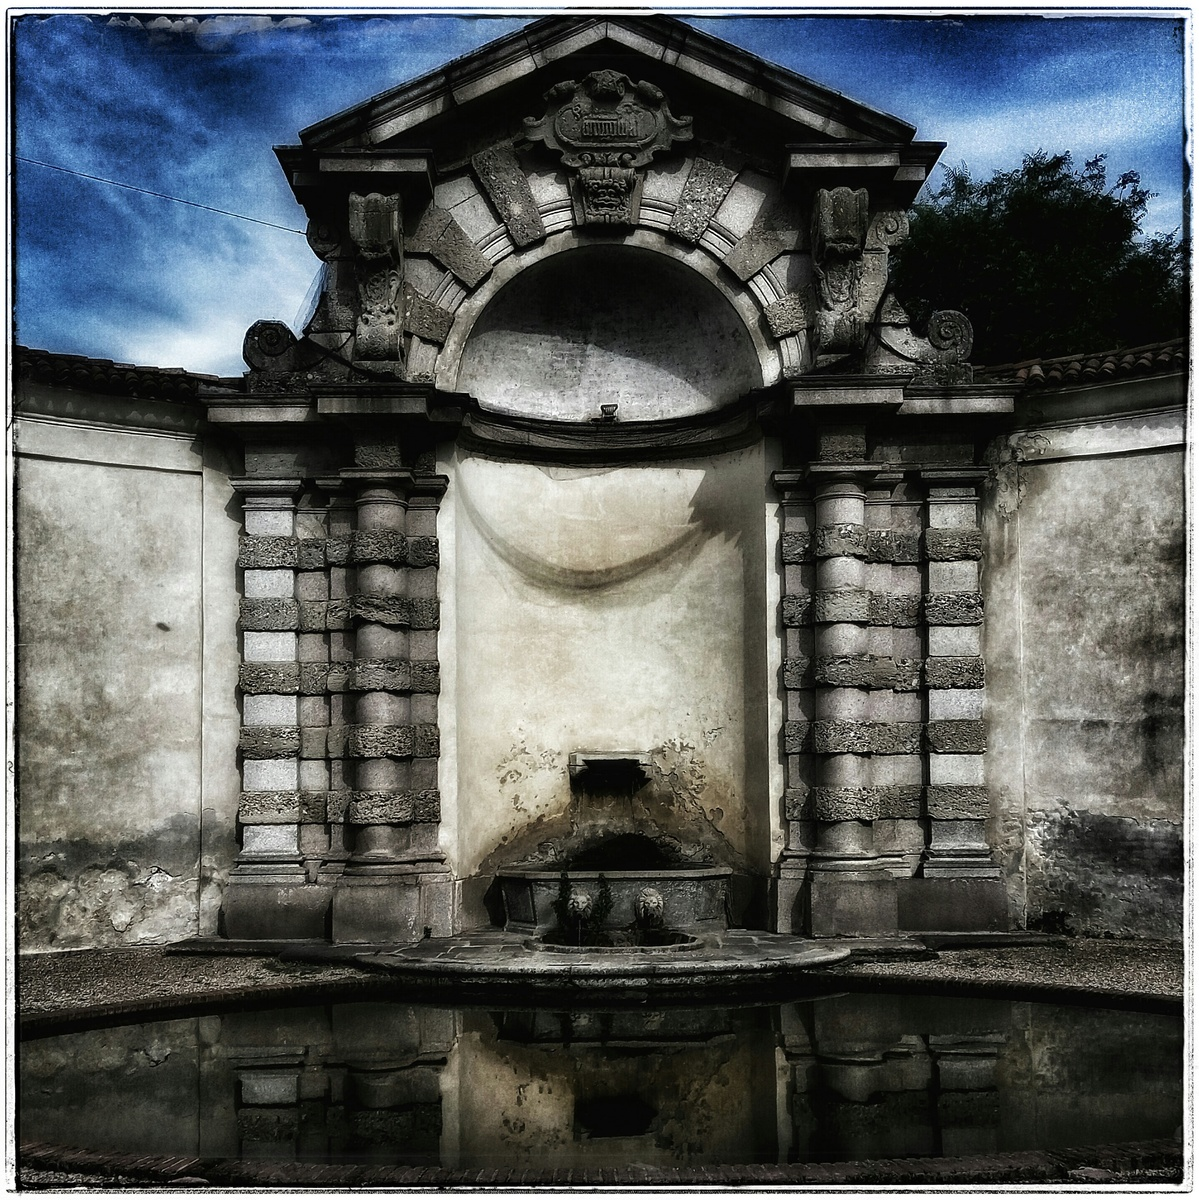
\includegraphics[width=0.8\linewidth]{thumb-lesson_IV.jpeg}
  %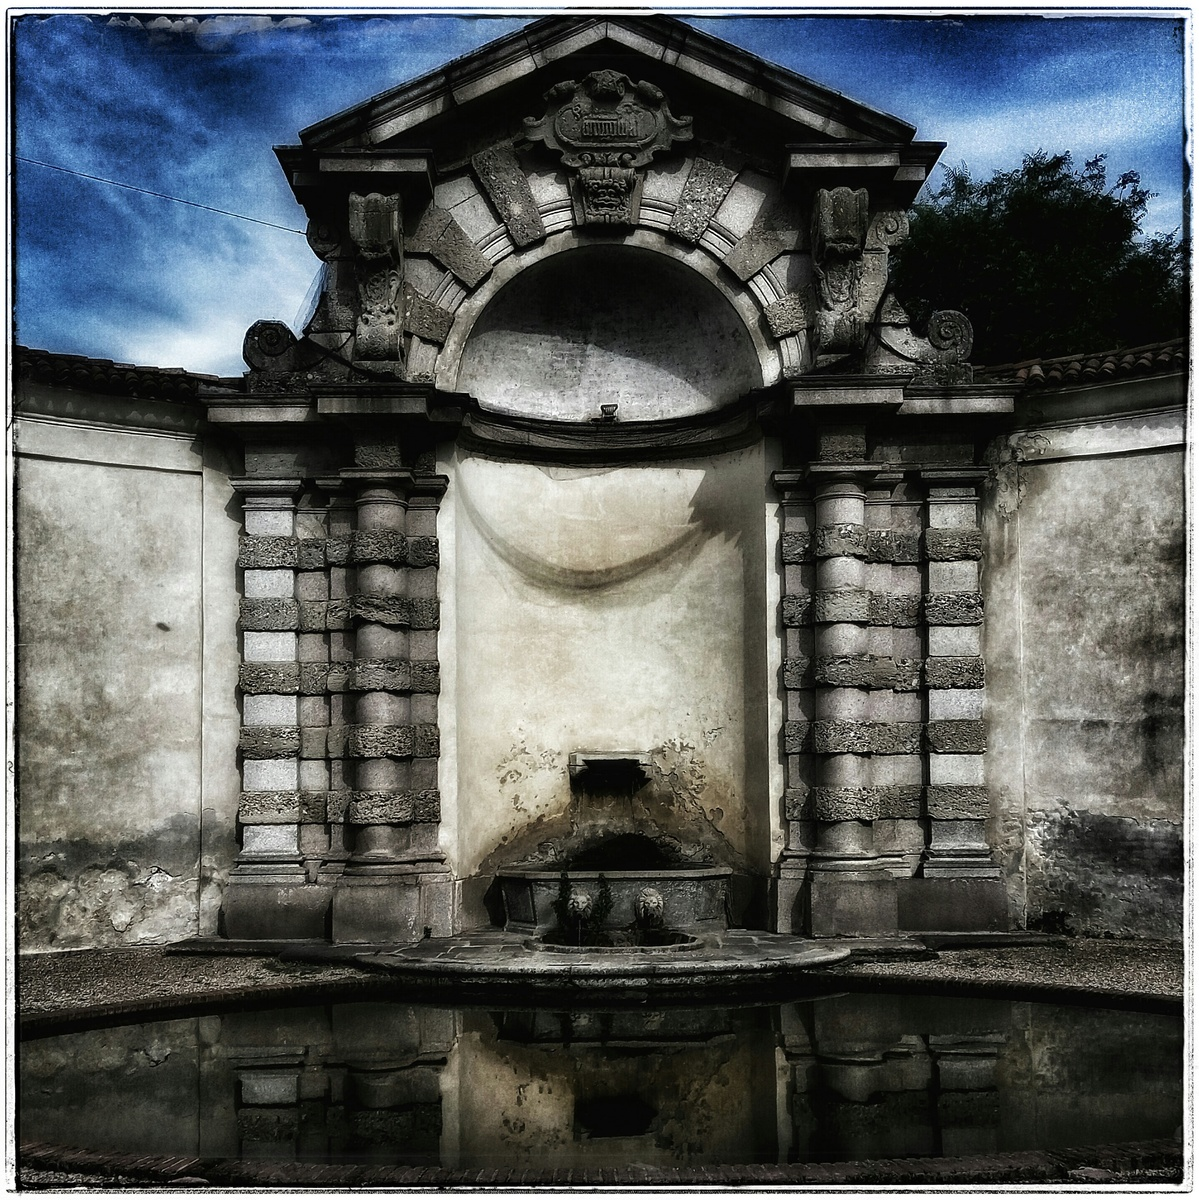
\includegraphics{thumb-lesson_IV.jpeg}
  \caption{Pavia: Almo Collegio Borromeo}
  \label{fig:textfig}
  %\zsavepos{pos:textfig}
  %\setfloatalignment{b}
\end{figure}

 

\nobibliography{latinBiblio}
\bibliographystyle{alpha}


\end{document}